\section{Modelling Customer Behaviours}
\label{sec:model}

Customers' behaviour evolves over time as they respond to business offering and adjust to their own demand. We would like to represent the various behaviour dynamics of a collection of customers by panel data, and employ the Markov chain model to describe these data. In addition, we use the mixture model to find Markov states, each of which defines a partition of the behaviours observable within a single time interval.

\subsection{Representing Behaviours by Features}

A \textit{feature} is an individual measurable property of a behaviour being observed, and choosing informative features is crucial for effective clustering. For example, to measure how often the pupil uses Whizz online tutorial, we can define the time spent or number of visits within a month as the feature. For each customer, we define multiple features to capture his behaviours of various aspects within a time interval. Suppose we are interested in studying bahaviours of $n$ customers in $T$ discrete consecutive time periods, and define $m$ features, then we denote the feature data as a sequence:
\begin{equation}
\label{eq:customerJourney}
\left\lbrace \mathbf{X}_1, ~\mathbf{X}_2, ~\dots, ~\mathbf{X}_t, ~\dots, ~\mathbf{X}_T \right\rbrace,
\end{equation}
in which the $t$-th element $\mathbf{X}_t = (x_{ij}^t) \in \mathbb{R}^{m \times n}$ is a matrix for all $t=1,2,\dots,T$. In addition, we denote the features of customer $j$ at the $t$-th time interval by the $j$-th column of $\mathbf{X}_t$ by $\mathbf{x}_{tj} = [x_{1j}^t ~x_{2j}^t ~\cdots ~x_{mj}^t]^\top$.

\subsection{Customer Journeys and Markov Chain}

Customer journeys reflect their feature dynamics over time, denoted as (\ref{eq:customerJourney}). One practical challenge of computing such sequence of matrices is to resolve the inconsistency present in journeys of different customers. The inconsistency refers to the problem that the time intervals for different customers being alive in the services are not aligned, so that their features are not comparable. Moreover, it is highly likely to have significant missing information within specific time intervals for customers who have not yet entered the service or have already churned. To resolve the inconsistency, we align and aggregate customers' features by \textit{customer month} rather than calendar month. Doing so enables the effective modelling using Markov chain.

\subsubsection{Customer Month}

Splitting pupils' behaviours into monthly time periods makes most sense provided the business settings at Whizz. Pupils subscribe to access Whizz products on a 1-month contract, and make the choice to leave the service at the end of each subscription. If no action is taken, a renewal will be made by default.

Due to the inconsistency present in journeys of different customers, we align their features by switching the reference from calendar month to customer month. This is illustrated by an example in \Cref{fig:customerMonth}. It provides much cleaner and more sensible data for modelling task. 

\begin{figure}[!h]
\centering
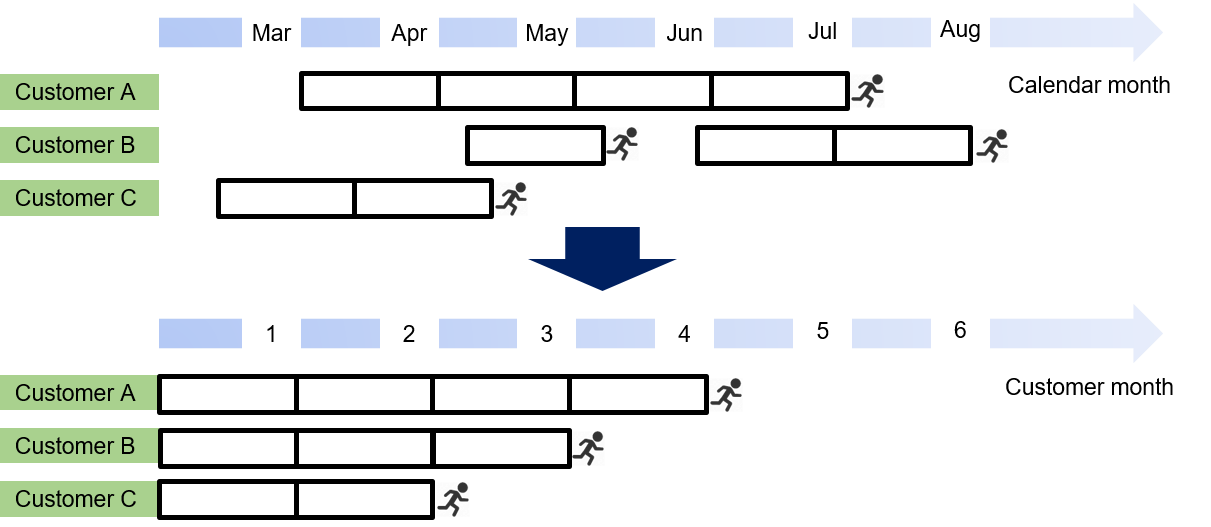
\includegraphics[scale=.75]{CustomerMonth.png}
\caption{Change reference from calendar month to customer month. Customer A, B and C have very different journeys in the sense of subscription start and end dates. Each block represents customer's monthly features. Under calendar month reference, we have to choose studying months from March to August to cover all activities. This choice results in irregular temporal distribution of missing information for all 3 customers. After changing the reference to customer month, features are aligned by customer month and therefore comparable. Moreover, the missing information only occurs after the customer churns. It can also handle discontinuous subscriptions like the case of customer B.}
\label{fig:customerMonth}
\end{figure}

\subsubsection{Markov Chain - Dynamic Model for Behavioural Changes}

We assume that customers with intentions to churn exhibit different behaviours than others do. Behaviours are different distributionally, and generated from a finite number of \textit{states}. Then the discrete time behaviour of each customer results in a chain of states over time. This formulates into a discrete-time Markov chain with states transiting over time, where each state emits distinguishable behaviour distribution from others. An example is given in \Cref{fig:markovChain}. In brief, a Markov chain is a stochastic process characterised by \textit{transition} and \textit{emission} probabilities.

\begin{figure}[!h]
\centering
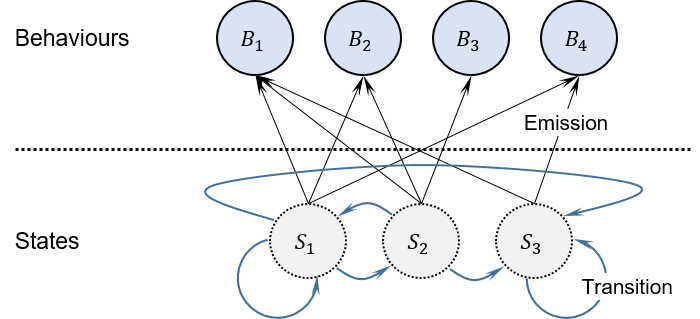
\includegraphics[scale=.75]{Markov.png}
\caption{Behaviours emitted from Markov states. States $S_1$, $S_2$ and $S_3$ generate differently distributed behaviours. For example, $S_1$ generates $\{ B_1, ~B_2, ~B_4\}$ while $S_3$ produces $\{ B_1, ~B_4\}$. Even if the two states can generate the same set of behaviours, the emission probabilities can be different, thus still resulting in different behaviour distributions. States transit between each other over time stochastically.}
\label{fig:markovChain}
\end{figure}

\paragraph*{Transition}

Consider the behavioural journey of customer $j$, which is represented by a sequence of feature data $\{ \mathbf{x}_{tj} \}_{t=1}^{T}$. At time interval $t$, feature $\mathbf{x}_{tj}$ is an instance from a distribution generated by a state. Let's denote the time sequence of generative states as $\{ s_{t}(j) \}_{t=1}^{T}$. In a Markov chain setting the sequences are defined stochastically, with the next state being conditionally dependent on the present state, but not any further previous history. This is known as \textit{Markov property}. 

If we define a finite set of states by $\mathcal{S} = \{ S_q \}_{q=1}^Q$, then $s_t (\cdot)$ is a map from $\mathbb{N}$ to $\mathcal{S}$. Due to the Markov property, successive states are linked together with the (conditional) \textit{transition probability matrix} defined as:
\begin{subequations}
\begin{equation}
A_t = (a_{pq}^t) \in [0,1]^{Q \times Q}, 
\end{equation}
with
\begin{equation}
a_{pq}^t = \mathbb{P} \left( s_{t+1} = S_p | s_t = S_q \right).
\end{equation}
\label{eq:transition}
\end{subequations}
If we assume time-homogeneity or \textit{stantionarity} of the Markov chain, then we can remove the time subscript from the notations because the parameters describing all probabilistic transitions are themselves constant.

\paragraph*{Emission}

Recall that feature data $\{ \mathbf{x}_{tj} \}_{t=1}^{T}$ observed are instances from some distribution. We introduce a generic notation for observed sequence of features, $\{ \mathbf{o}_{t} \}_{t=1}^{T}$, where $\mathbf{o}_t = [o_{t1} ~o_{t2} ~\cdots ~o_{tm}]^\top$. The sequence of observations are generated in the following way:
\begin{enumerate}
\item At each time step, the system generates a state $s_t$ according to the state-to-state transition probability matrix $A_t$.
\item Once the state $s_t$ has been generated, the system generates a cluster $c_t$ according to a state-to-cluster emission probability distribution $\pi(s_t,c_t)$. Suppose we define a finite collection of clusters $\mathcal{C} = \{ C_k \}_{k=1}^K$, then we denote:
\begin{equation}
\pi_{qk} = \pi(S_q, C_k) = \mathbb{P} \left( c_t = C_k | s_t = S_q \right).
\end{equation}
\item Once the cluster $c_t$ have been determined, an observation vector $\mathbf{o}_t$ is produced probabilistically according to some cluster-specific distribution $\phi(\mathbf{o}_t | \theta (s_t, c_t))$, where $\theta (s_t, c_t)$ denotes the distribution parameters. We write,
\begin{equation}
\phi(\mathbf{o}_t ; \theta_{qk}) =  \phi(\mathbf{o}_t ; \theta (S_q, C_k)) = \mathbb{P} \left( \mathbf{o}_t | s_t = S_q, c_t = C_k \right).
\end{equation}
\end{enumerate}
Given the generative process described above, we can now model the state-to-observation emission probability by a mixture of densities:
\begin{subequations}
\begin{align}
b_q (\mathbf{o}_t) & = \mathbb{P} \left( \mathbf{o}_t | s_t = S_q \right) \\
 & = \sum_{k=1}^K  \mathbb{P} \left( c_t = C_k | s_t = S_q \right) \mathbb{P} \left( \mathbf{o}_t | s_t = S_q, c_t = C_k \right) \\
 & = \sum_{k=1}^K \pi_{qk} \phi(\mathbf{o}_t ; \theta_{qk}).
\end{align}
\label{eq:emission}
\end{subequations}

\subsubsection{Decoding the Markov Chain}

The problem is how to estimate the transition probabilities and parameters in the emission term, $A_t$ and $(\pi, \theta)$ from the observations $\mathbf{X}_t$. Our strategy is to split this decoding process into two separate steps, where we first make inference on emission and then uncover the temporal structure configured by transition.

\paragraph*{Decoding Emission}

Ideally from the perspective of practical application of the model, we wish to encode a finite number of states representing different levels of churn risk. As a consequence, the prediction task is to find out the state that the pupil belongs to and therefore assigning the associated risk label. Hence, we choose not to infer states purely from observed behavioural data, but define states by also incorporating churn outcome information. At high level, we take two steps to estimate the parameters in the emission term:
\begin{enumerate}
\item We look at the behavioural distribution without conditioning on state, namely,
\begin{equation}
b(\mathbf{o}_t) = \mathbb{P} (\mathbf{o}_t) = \sum_{k=1}^K \mathbb{P} (c_t = C_k) \mathbb{P} (\mathbf{o}_t | c_t = C_k) = \sum_{k=1}^K \pi_k \phi(\mathbf{o}_t ; \theta_k).
\end{equation}
Then we estimate $\{ \pi_k, \theta_k \}_{k=1}^K$ from observed feature data $\mathbf{X}_t$ with pre-defined multivariate kernel density $\phi(\cdot)$. This will be elaborated in section \ref{sec:mixtureModel}.

\item The previous step gives not only the weights $\pi$ and cluster density $\phi(\cdot | \theta)$, but also a consequential cluster assignment of all customers. If we know the churn outcome for all customers, then we can calculate the proportion of churned customers, or churn rate, within each cluster. Thereafter, we can form states by grouping together clusters of similar level of churn rate.

Formally, we define the set of customers who have been assigned into cluster $C_k$ as
\begin{equation}
\mathcal{N}_k^t = \left\lbrace j :~ j \text{ is assigned into } C_k \text{ at time } t \right\rbrace.
\end{equation}
Meanwhile, we define the churn outcome information by a set
\begin{equation}
\mathcal{N}_\text{churn}^t = \{j: ~j \text{ churns at } t+1 \},
\end{equation}
so that the cluster churn rate is defined as
\begin{equation}
\lambda_k^t = \frac{\vert \mathcal{N}_k^t \cap \mathcal{N}_\text{cancel}^t \vert}{\vert  \mathcal{N}_k^t \vert}.
\end{equation}
Once the churn rates of all $K$ clusters, $\{ \lambda_k^t \}_{k=1}^K$, are computed, we group them and form $Q$ states. Typically $Q$ is much smaller than $K$. We denote the set of clusters consisting state $S_q$ as,
\begin{equation}
\mathcal{K}_q^t = \left\lbrace k :~ C_k \text{ is emitted from } S_q \text{ at time } t \right\rbrace.
\end{equation}
\end{enumerate}
Afterwards, we can revisit the calculation for the state-to-observation emission probability $b_q(\mathbf{o}_t)$. Note that by the way we define state, we have
\begin{equation}
\pi_{qk} = \mathbb{P} \left( c_t = C_k | s_t = S_q \right) = \frac{\vert \mathcal{N}_k^t \vert}{\sum_{l \in \mathcal{K}_q^t} \vert \mathcal{N}_l^t \vert} \mathbbm{1}_{\{ k \in \mathcal{K}_q^t \}},
\end{equation}
where $\mathbbm{1}_{\{\cdot\}}$ is the indicator function. Then
\begin{equation}
b_q (\mathbf{o}_t) = \sum_{k=1}^K \pi_{qk} \phi(\mathbf{o}_t ; \theta_{qk}) = \sum_{ k \in \mathcal{K}_q^t } \frac{\vert \mathcal{N}_k^t \vert}{\sum_{l \in \mathcal{K}_q^t} \vert \mathcal{N}_l^t \vert} \phi(\mathbf{o}_t ; \theta_{k}).
\end{equation}

\paragraph*{Decoding Transition}

We define the set of customers who transit from $S_p$ at $t$ to $S_q$ at $t+1$ as
\begin{equation}
\mathcal{Q}_{q \rightarrow p}^t = \left\lbrace j: ~s_t(j) = S_q, ~s_{t+1}(j) = S_p \right\rbrace.
\end{equation}
We assume that customers' behaviours are independent from others, then the maximum likelihood estimate of the transition probability is
\begin{equation}
\hat{a}^t_{pq} = \frac{\vert \mathcal{Q}_{q \rightarrow p}^t \vert}{\sum_{l=1}^Q \vert \mathcal{Q}_{q \rightarrow l}^t \vert}.
\end{equation}
If the Markov chain is assumed to be stationary, then we estimate
\begin{equation}
\hat{a}_{pq} = \frac{\sum_{t=1}^T \vert \mathcal{Q}_{q \rightarrow p}^t \vert}{\sum_{t=1}^T \sum_{l=1}^Q \vert \mathcal{Q}_{q \rightarrow l}^t \vert}.
\end{equation}










\subsection{Probabilistic Clustering Using Mixture Model}
\label{sec:mixtureModel}

\paragraph{Generative process}

\begin{equation}
\mathbb{P} (\mathbf{y}, \mathbf{c}, \bm \theta) = \prod_{k=1}^K G_0 (\theta_k) \prod_{n=1}^N F(y_n | \theta_{c_n}) P(c_n)
\end{equation}

\begin{itemize}
\item $\mathbf{y} = \{y_1, y_2, \cdots, y_N \}$, observations
\item $\mathbf{c} = \{c_1, c_2, \cdots, c_N \}$, cluster assignments
\item $\bm \theta = \{\theta_1, \theta_2, \cdots, \theta_K \}$, cluster parameters
\item $G_0(\theta)$, a prior over the cluster parameters
\item $P(c)$, a prior over the mixing distribution
\item $F(y_n|\theta_{c_n})$, a hypothetical distribution over the observations
\item Assumptions: each observation is conditionally independent given its latent cluster assignments and the cluster parameters
\end{itemize}

\paragraph{Posterior probability of assignments}

\begin{equation}
\mathbb{P} (\mathbf{c} | \mathbf{y}) = \frac{\mathbb{P}(\mathbf{y} | \mathbf{c}) P(\mathbf{c})}{\sum_{\mathbf{c}} \mathbb{P}(\mathbf{y} | \mathbf{c}) P(\mathbf{c})},
\end{equation}
where
\begin{equation}
\mathbb{P}(\mathbf{y} | \mathbf{c}) = \int_\theta \left[ \prod_{n=1}^N F(y_n | \theta_{c_n}) \prod_{k=1}^K G_0 (\theta_k) \right] \text{d} \theta
\end{equation}


BNP clustering assume that there is an infinite number of latent clusters (namely $K \rightarrow +\infty$), but that a finite number of them is used to generate the observed data. There are an infinite number of clusters, though a finite data set only exhibits a finite number of active clusters.

\subsection{Modelling Pipeline}

Feature extraction

Features distributional modelling

Fitting mixture model

Analytic (churn rate calculation, clusters interpretation)